\label{sec:appendix}

\begin{table}
\centering
\small
\renewcommand{\arraystretch}{1.3}

\begin{tabular}{c|c|c|c}
\toprule
Constraint & String & Feature & AR \\
\midrule

\textbf{\textsc{*Rise$_\sigma$}} 
& LH
& \begin{tabular}{@{}rcc@{}}
  L: & $+$ & $-$ \\
  C: & $-$ & $-$ \\
  B: & $0$ & $0$
  \end{tabular}
&
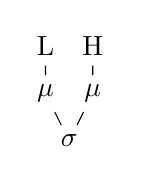
\begin{tikzpicture}[scale=.6, baseline=(current bounding box.center)]
  \node (t1) at (0,1) {L};
  \node (t2) at (1,1) {H};
  \node (m1) at (0,0) {$\mu$};
  \node (m2) at (1,0) {$\mu$};
  \node (s1) at (.5,-1) {$\sigma$};
  \draw (t1)--(m1)--(s1);
  \draw (t2)--(m2)--(s1);
\end{tikzpicture} \\

\midrule

\multirow[b]{3}{*}{\textbf{\textsc{*Contour$_{\mu}$}}}
& R
& \begin{tabular}{@{}rc@{}}
  L: & $+$ \\
  C: & $+$ \\
  B: & $0$
  \end{tabular}
&
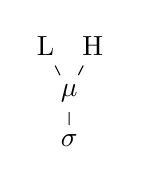
\begin{tikzpicture}[scale=.6, baseline=(current bounding box.center)]
  \node (t1) at (0,1) {L};
  \node (t2) at (1,1) {H};
  \node (m1) at (.5,0) {$\mu$};
  \node (s1) at (.5,-1) {$\sigma$};
  \draw (t1)--(m1)--(s1);
  \draw (t2)--(m1);
\end{tikzpicture} \\
\cmidrule{2-4}

& F
& \begin{tabular}{@{}rc@{}}
  L: & $-$ \\
  C: & $+$ \\
  B: & $0$
  \end{tabular}
&
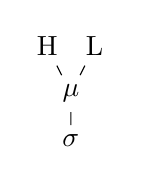
\begin{tikzpicture}[scale=.6, baseline=(current bounding box.center)]
  \node (t1) at (0,1) {H};
  \node (t2) at (1,1) {L};
  \node (m1) at (.5,0) {$\mu$};
  \node (s1) at (.5,-1) {$\sigma$};
  \draw (t1)--(m1)--(s1);
  \draw (t2)--(m1);
\end{tikzpicture} \\

\midrule

& HHH
& \begin{tabular}{@{}rccc@{}}
  L: & $-$ & $-$ & $-$ \\
  C: & $-$ & $-$ & $-$ \\
  B: & $0$ & $0$ & $0$
  \end{tabular}
& \\

\cmidrule{2-3}

& LLL
& \begin{tabular}{@{}rccc@{}}
  L: & $+$ & $+$ & $+$ \\
  C: & $-$ & $-$ & $-$ \\
  B: & $0$ & $0$ & $0$
  \end{tabular}
& \\

\cmidrule{2-3}

\textbf{\textsc{*3T} 
}& HHL
& \begin{tabular}{@{}rccc@{}}
  L: & $-$ & $-$ & $+$ \\
  C: & $-$ & $-$ & $-$ \\
  B: & $0$ & $0$ & $0$
  \end{tabular}
& 
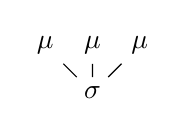
\begin{tikzpicture}[scale=.6, baseline=(current bounding box.center)]
  \node (m1) at (0,0) {$\mu$};
  \node (m2) at (1,0) {$\mu$};
  \node (m3) at (2,0) {$\mu$};
  \node (s1) at (1,-1) {$\sigma$};
  \draw (m1)--(s1);
  \draw (m2)--(s1);
  \draw (m3)--(s1);
\end{tikzpicture} \\
\cmidrule{2-3}

& HLL
& \begin{tabular}{@{}rccc@{}}
  L: & $-$ & $+$ & $+$ \\
  C: & $-$ & $-$ & $-$ \\
  B: & $0$ & $0$ & $0$
  \end{tabular}
&  \\

\cmidrule{2-3}

& HLH
& \begin{tabular}{@{}rccc@{}}
  L: & $-$ & $+$ & $-$ \\
  C: & $-$ & $-$ & $-$ \\
  B: & $0$ & $0$ & $0$
  \end{tabular}
& \\

\midrule

\textbf{\textsc{*NoFinHL}}
& HL.
& \begin{tabular}{@{}rccc@{}}
  L: & $-$ & $+$ & $0$ \\
  C: & $-$ & $-$ & $0$ \\
  B: & $0$ & $0$ & $+$
  \end{tabular}
&
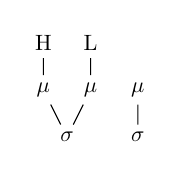
\begin{tikzpicture}[scale=0.6, every node/.style={scale=0.8}, baseline=(current bounding box.base)]
  \node (t0) at (1,1) {H};
  \node (t1) at (2,1) {L};
  \node (c1) at (1,0) {$\mu$};
  \node (c2) at (2,0) {$\mu$};
  \node (c3) at (3,0) {$\mu$};
  \node (s1) at (1.5,-1) {$\sigma$};
  \node (s2) at (3,-1) {$\sigma$};
  \draw (t0) -- (c1) -- (s1);
  \draw (t1) -- (c2) -- (s1);
  \draw (c3) -- (s2);
\end{tikzpicture} \\

\midrule

\textbf{\textsc{*Lapse}}
& L.L
& \begin{tabular}{@{}rccc@{}}
  L: & $+$ & $0$ & $+$ \\
  C: & $-$ & $0$ & $0$ \\
  B: & $0$ & $+$ & $0$
  \end{tabular}
&
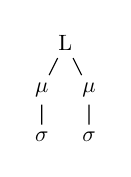
\begin{tikzpicture}[scale=0.6, every node/.style={scale=0.8}, baseline=(current bounding box.base)]
  \node (t1) at (1.5,1) {L};
  \node (c1) at (1,0) {$\mu$};
  \node (c2) at (2,0) {$\mu$};
  \node (s1) at (1,-1) {$\sigma$};
  \node (s2) at (2,-1) {$\sigma$};
  \draw (t1) -- (c1) -- (s1);
  \draw (t1) -- (c2) -- (s2);
\end{tikzpicture} \\

\bottomrule
\end{tabular}

\caption{Baseline constraints represented in string, feature, and autosegmental representations. Note: the string and featural representations for \textsc{*3T} would also include LHH, LHL, and LLH, but these patterns are ruled out by \textsc{*Rise$_{\mu}$}.}
\end{table}